\ifx\wholebook\relax \else
% ------------------------ 

\documentclass{article}
%------------------- Other types of document example ------------------------
%
%\documentclass[twocolumn]{IEEEtran-new}
%\documentclass[12pt,twoside,draft]{IEEEtran}
%\documentstyle[9pt,twocolumn,technote,twoside]{IEEEtran}
%
%-----------------------------------------------------------------------------
%%
% loading packages
%
\newif\ifpdf
\ifx\pdfoutput\undefined % We're not running pdftex
  \pdffalse
\else
  \pdftrue
\fi
%
%
\ifpdf
  \RequirePackage[pdftex,%
            CJKbookmarks,%
       bookmarksnumbered,%
              colorlinks,%
          linkcolor=blue,%
              hyperindex,%
        plainpages=false,%
       pdfstartview=FitH]{hyperref}
\else
  \RequirePackage[dvipdfm,%
             CJKbookmarks,%
        bookmarksnumbered,%
               colorlinks,%
           linkcolor=blue,%
               hyperindex,%
         plainpages=false,%
        pdfstartview=FitH]{hyperref}
  \AtBeginDvi{\special{pdf:tounicode GBK-EUC-UCS2}} % GBK -> Unicode
\fi
\usepackage{hyperref}

% other packages
%-----------------------------------------------------------------------------
\usepackage{graphicx, color}
\usepackage{CJK}
%
% for programming 
%
\usepackage{verbatim}
\usepackage{listings}


\lstdefinelanguage{Smalltalk}{
  morekeywords={self,super,true,false,nil,thisContext}, % This is overkill
  morestring=[d]',
  morecomment=[s]{"}{"},
  alsoletter={\#:},
  escapechar={!},
  literate=
    {BANG}{!}1
    {UNDERSCORE}{\_}1
    {\\st}{Smalltalk}9 % convenience -- in case \st occurs in code
    % {'}{{\textquotesingle}}1 % replaced by upquote=true in \lstset
    {_}{{$\leftarrow$}}1
    {>>>}{{\sep}}1
    {^}{{$\uparrow$}}1
    {~}{{$\sim$}}1
    {-}{{\sf -\hspace{-0.13em}-}}1  % the goal is to make - the same width as +
    %{+}{\raisebox{0.08ex}{+}}1		% and to raise + off the baseline to match -
    {-->}{{\quad$\longrightarrow$\quad}}3
	, % Don't forget the comma at the end!
  tabsize=2
}[keywords,comments,strings]

\lstloadlanguages{C++, Lisp, Smalltalk}

% ======================================================================

\def\BibTeX{{\rm B\kern-.05em{\sc i\kern-.025em b}\kern-.08em
    T\kern-.1667em\lower.7ex\hbox{E}\kern-.125emX}}

\newtheorem{theorem}{Theorem}

%
% mathematics
%
\newcommand{\be}{\begin{equation}}
\newcommand{\ee}{\end{equation}}
\newcommand{\bmat}[1]{\left( \begin{array}{#1} }
\newcommand{\emat}{\end{array} \right) }
\newcommand{\VEC}[1]{\mbox{\boldmath $#1$}}

% numbered equation array
\newcommand{\bea}{\begin{eqnarray}}
\newcommand{\eea}{\end{eqnarray}}

% equation array not numbered
\newcommand{\bean}{\begin{eqnarray*}}
\newcommand{\eean}{\end{eqnarray*}}

\RequirePackage{CJK,CJKnumb,CJKulem,CJKpunct}
% we use CJK as default environment
\AtBeginDocument{\begin{CJK*}{GBK}{song}\CJKtilde\CJKindent\CJKcaption{GB}}
\AtEndDocument{\clearpage\end{CJK*}}

%
% loading packages
%
\newif\ifpdf
\ifx\pdfoutput\undefined % We're not running pdftex
  \pdffalse
\else
  \pdftrue
\fi
%
%
\ifpdf
  \RequirePackage[pdftex,%
       bookmarksnumbered,%
              colorlinks,%
          linkcolor=blue,%
              hyperindex,%
        plainpages=false,%
       pdfstartview=FitH]{hyperref}
\else
  \RequirePackage[dvipdfm,%
        bookmarksnumbered,%
               colorlinks,%
           linkcolor=blue,%
               hyperindex,%
         plainpages=false,%
        pdfstartview=FitH]{hyperref}
\fi
\usepackage{hyperref}

% other packages
%-----------------------------------------------------------------------------
\usepackage{graphicx, color}
%
% for programming 
%
\usepackage{verbatim}
\usepackage{listings}
\usepackage{algorithmic} %for pseudocode
\usepackage{algorithm}


\lstdefinelanguage{Smalltalk}{
  morekeywords={self,super,true,false,nil,thisContext}, % This is overkill
  morestring=[d]',
  morecomment=[s]{"}{"},
  alsoletter={\#:},
  escapechar={!},
  literate=
    {BANG}{!}1
    {UNDERSCORE}{\_}1
    {\\st}{Smalltalk}9 % convenience -- in case \st occurs in code
    % {'}{{\textquotesingle}}1 % replaced by upquote=true in \lstset
    {_}{{$\leftarrow$}}1
    {>>>}{{\sep}}1
    {^}{{$\uparrow$}}1
    {~}{{$\sim$}}1
    {-}{{\sf -\hspace{-0.13em}-}}1  % the goal is to make - the same width as +
    %{+}{\raisebox{0.08ex}{+}}1		% and to raise + off the baseline to match -
    {-->}{{\quad$\longrightarrow$\quad}}3
	, % Don't forget the comma at the end!
  tabsize=2
}[keywords,comments,strings]

\lstloadlanguages{C++, Lisp, Haskell, Python, Smalltalk}

% ======================================================================

\def\BibTeX{{\rm B\kern-.05em{\sc i\kern-.025em b}\kern-.08em
    T\kern-.1667em\lower.7ex\hbox{E}\kern-.125emX}}

\newtheorem{theorem}{Theorem}

%
% mathematics
%
\newcommand{\be}{\begin{equation}}
\newcommand{\ee}{\end{equation}}
\newcommand{\bmat}[1]{\left( \begin{array}{#1} }
\newcommand{\emat}{\end{array} \right) }
\newcommand{\VEC}[1]{\mbox{\boldmath $#1$}}

% numbered equation array
\newcommand{\bea}{\begin{eqnarray}}
\newcommand{\eea}{\end{eqnarray}}

% equation array not numbered
\newcommand{\bean}{\begin{eqnarray*}}
\newcommand{\eean}{\end{eqnarray*}}




\setcounter{page}{1}

\begin{document}

\fi
%--------------------------

% ================================================================
%                 COVER PAGE
% ================================================================

\title{Suffix Tree with Functional and imperative implementation}

\author{Liu~Xinyu
\thanks{{\bfseries Liu Xinyu } \newline
  Email: liuxinyu95@gmail.com \newline}
%  Tel:   +86-1305-196-8666 \newline}
  }

\markboth{Suffix Tree}{Imperative and Functional}

\maketitle

\ifx\wholebook\relax
\chapter{Suffix Tree with Functional and imperative implementation}

\section{abstract}
\else
\begin{abstract}
\fi
Suffix Tree is an important data structure. It is quite powerful in 
string and DNA informaiton manipulations. Suffix Tree is introduced in 1973.
The latest online construction algorithm was found in 1995. This post 
collects some existing result of suffix tree, including the construction
algorithms as well as some typical applications. Some imperative and functional
implementation are given. There are multiple programming languages used, 
including C++, Haskell, Python and Scheme/Lisp.

There may be mistakes in the post, please feel free to point out.

This post is generated by \LaTeXe, and provided with GNU FDL(GNU Free Documentation License).
Please refer to http://www.gnu.org/copyleft/fdl.html for detail.

\ifx\wholebook\relax \else
\end{abstract}
\fi

\vspace{3cm}
{\bfseries Keywords:} Suffix Tree

%{\bfseries Corresponding Author:} Liu Xinyu

\maketitle

% ================================================================
%                 Introduction
% ================================================================
\section{Introduction}
\label{introduction}

Suffix Tree is a special Patricia. There is no such a chapter
in CLSR book. To introduce suffix tree together with Trie and Patricia
will be a bit easy to understand. 

As a data structure, Suffix tree allows for paticulary fast implementation
of many important string operations\cite{wiki-suffix-tree}. And it is 
also widely used in bio-information area such as DNA pattern 
matching\cite{ukkonen-presentation}.

The suffix tree for a string $S$ is a Patricia tree, with each edges are labeled
with some sub-string of $S$. Each suffix of $S$ corresponds to exactly one path
from root to a leaf. Figure \ref{fig:stree-banana} shows the suffix tree for
an English word `banana'.

\begin{figure}[htbp]
       \begin{center}
	\includegraphics[scale=0.5]{img/stree-banana.ps}
        \caption{The suffix tree for `banana'} \label{fig:stree-banana}
       \end{center}
\end{figure}

Note that all suffixes, 'banana', 'anana', 'nana', 'ana', 'na', 'a', '' can 
be looked up in the above tree. Among them the first 3 suffixes are explicitly
shown; others are implicitly represented. The reason for why 'ana, 'na', 'a', 
and '' are not shown explicitly is because they are prefixes of some edges.
In order to make all suffixes shown explicitly, we can append a special pad 
terminal symbal, which is not seen to the string. Such terminator is typically
denoted as '\$'. With this method, no suffix will be a prefix of the others.
In this post, we won't use terminal symbol for most cases.

It's very interesting that compare to the simple suffix tree for 'banana', the
suffix tree for 'bananas' is quite different as shown in figure \ref{fig:stree-bananas}.

\begin{figure}[htbp]
       \begin{center}
	\includegraphics[scale=0.5]{img/stree-bananas.ps}
        \caption{The suffix tree for `bananas'} \label{fig:stree-bananas}
       \end{center}
\end{figure}

In this post, I'll first introduce about suffix Trie, and give the trivial method
about how to construct suffix Trie and tree. Trivial methods utilize the insertion
algorithm for normal Trie and patricia. They need much of computation and spaces.
Then, I'll explain about the online construction for suffix Trie by using suffix link
concept. After that, I'll show Ukkonen's method, which is a linear time online 
construction algorithm. For both suffix Trie and suffix tree, functional approach
is provided as well as the imperative one. In the last section, I'll list some
typical string manipulation problems and show how to solve them with suffix tree.

This article provides example implementation in C, C++, Haskell, Python, and 
Scheme/Lisp languages. 

All source code can be downloaded in appendix \ref{appendix}, please 
refer to appendix for detailed information about build and run.

% ================================================================
%                 Suffix Trie
% ================================================================
\section{Suffix Trie}
\label{suffix-trie}

Just likes the relationship between Trie and Patricia, Suffix Trie has much simpler
structure than suffix tree. Figure \ref{fig:strie-banana} shows the suffix Trie of
'banana'.

\begin{figure}[htbp]
       \begin{center}
	\includegraphics[scale=0.5]{img/strie-banana.ps}
        \caption{Suffix Trie of 'banana'} \label{fig:strie-banana}
       \end{center}
\end{figure}

Compare with figure \ref{fig:stree-banana}, the difference is that, instead of representing
a word for each edge, one edge in suffix Trie only represents one character. Thus
suffix Trie need more spaces. If we pack all nodes which has only one child, the suffix
Trie can be turned into a suffix tree.

Suffix Trie can be a good start point for explaining the suffix tree construction algorithm.

%=========================================================================
%       Trivial construction of Suffix Trie and Suffix Tree
%=========================================================================
\subsection{Trivial construction methods of Suffix Tree}
\label{trivial-cons}

By repeatly applying the insertion algorithms\cite{lxy-trie} for Trie and Patricia
on each suffixes of a word, Suffix Trie and tree can be built in a trivial way.

Below algorithm illustrates this approach for suffix tree.

\begin{algorithmic}
\STATE $TRIVIAL-SUFFIX-TREE(S)$
  \STATE $T \leftarrow NIL$
  \FOR{$i$ from $1$ to $LENGTH(S)$}
    \STATE $T \leftarrow PATRICIA-INSERT(T, RIGHT(S, i))$
  \ENDFOR
  \RETURN $T$
\end{algorithmic}

Where function $RIGHT(S, i)$ will extract substring of S from left to right most.
Similar functional algorithm can also be provided in this way.

\begin{algorithmic}
\STATE $TRIVIAL-SUFFIX-TREE'(S)$
  \RETURN $FOLD-LEFT(PATRICIA-INSERT, NIL, TAILS(S))$
\end{algorithmic}

Function TAILS() returns a list of all suffixes for string S. In Haskell, Module 
Data.List provides this function already. In Scheme/Lisp, it can be implemented as below.

\lstset{language=lisp}
\begin{lstlisting}
(define (tails s)
  (if (string-null? s)
      '("")
      (cons s (tails (string-tail s 1)))))
\end{lstlisting}

The trivial suffix Trie/tree construction method takes $O(n^2)$ time, where $n$ is the 
length of the word. Altough the string manipulation can be very fast by using suffix
tree, slow construction will be the bottleneck of the whole process.

% ================================================================
%               Online construction of Suffix Trie
% ================================================================
\subsection{Online construction of suffix trie}

Analysis of construction for suffix Trie can be a good start point in finding
the linear time suffix tree construction algorithm. In Ukkonen's paper\cite{ukkonen95}, 
finite-state automation, transition function and suffix function are used to 
build the mathematical model for suffix Trie/tree. 

In order to make it easy for understanding, let's explain the above concept with
the elements of Trie data structure.

With a set of alphabetic, a string with length $n$ can be defined as $S=s_1s_2...s_n$.
And we define $S[i]=s_1s_2...s_i$, which contains the first $i$ characters.

In a suffix Trie, each node represents a suffix string. for example in figure 
\ref{fig:strie-cacao}, node X represents suffix 'a', by adding a character 'c',
node X transfers to node Y which represents suffix 'ac'. We say node X and edge labelled 'c'
transfers to node Y. This relationship can be denoted in psuedo code as below.

\begin{figure}[htbp]
   \begin{center}
     \includegraphics[scale=0.4]{img/strie-cacao.ps}
     \caption{node $X \leftarrow$ ``a'', node $Y \leftarrow$ ``ac'', $X$ transfers to $Y$ with character 'c'}
     \label{fig:strie-cacao}
   \end{center}
\end{figure}

$Y \leftarrow CHILDREN(X)[c]$

It's equal to the following C++ and Python code.

\lstset{language=python}
\begin{lstlisting}
y = x.children[c]
\end{lstlisting}

We also say that node x has a c-child y.

If a node $A$ in a suffix Trie represents for a suffix $s_is_{i+1}...s_n$, 
and node $B$ represents for suffix $s_{i+1}s_{i+2}...s_n$, we say node $B$
represents for the suffix of node $A$. We can create a link from $A$ to $B$.
This link is defined as the suffix link of node $A$. In this post, we show
suffix link in dotted style. In figure \ref{fig:strie-cacao}, suffix link of
node $A$ points to node $B$, and suffix link of node $B$ points to node $C$.
Suffix link is an important tool in Ukkonen's online construction algorithm,
it is also used in some other algorithms running on the suffix tree.

\subsubsection{on-line construction algorithm for suffix Trie}
For a string $S$, Suppose we have construct suffix Trie for its $i$-th prefix
$s_1s_2...s_i$. We denote the suffix Trie for this $i$-th prefix as $SuffixTrie(S_i)$.
Let's consider how can we obtain $SuffixTrie(S_{i+1})$ from $SuffixTrie(S_i)$.

If we list all suffixes corresponding to $SuffixTrie(S_i)$, fromt the longest 
$S_i$ to the shortest empty string, we get table \ref{tab:suffixes_s_i}. There
are total $i+1$ suffixes.

\begin{table}
  \begin{tabular}{r}
    suffix string \\
    $s_1s_2...s_i$ \\
    $s_2s_3...s_i$ \\
    ... \\
    $s_{i-1}s_i$ \\
    $s_i$ \\
    ``'' \\
  \end{tabular}
  \caption{suffixes for $S_i$}
  \label{tab:suffixes_s_i}
\end{table}

The most straightforward way is to append $s_{i+1}$ to each of the suffix in above
table, and add a new empty suffix. This operation can be implemented as create
a new node, and append the new node as a child with edge bind to character $s_{i+1}$.

\begin{algorithm}
\begin{algorithmic}
\FOR{each $node$ in $SuffixTrie(S_i)$}
  \STATE $CHILDREN(node)[s_{i+1}] \leftarrow CREATE-NEW-NODE()$
\ENDFOR
\end{algorithmic}
\caption{Initial version of update $SuffixTrie(S_i)$ to $SuffixTrie(S_{i+1})$.}
\label{algo:strie1}
\end{algorithm}

However, some node in $SuffixTrie(S_i)$ may have already $s_{i+1}$-child. 
For example, in figure \ref{fig:strie-cac}, Node $X$ and $Y$ are corresonding 
for suffix 'cac' and 'ac', they don't have 'a'-child.
While node $Z$, which represents for suffix 'c' has 'a'-child already.

\begin{figure}[htbp]
   \begin{center}
     \includegraphics[scale=0.5]{img/strie-cac.ps}
     \includegraphics[scale=0.5]{img/strie-caca.ps}
     \caption{Suffix Trie of ``cac'' and ``caca''}
     \label{fig:strie-cac}
   \end{center}
\end{figure}

When we append $s_{i+1}$, in this case it is 'a', to $SuufixTrie(S_i)$. We need create
a new node and append the new node to $X$ and $Y$, however, we needn't create new
node to $Z$, because node $Z$ has already a child node with edge 'a'. So 
$SuffixTrie(S_{i+1})$, in this case it is for ``caca'', is shown in right part of
figure \ref{fig:strie-cac}.

If we check each node as the same order as in table \ref{tab:suffixes_s_i}, we can 
stop immediately once we find a node which has a $s_{i+1}$-child. This is because 
if a node $X$ in $SuffixTrie(S_i)$ has already a $s_{i+1}$-child, then according to the
definition of suffix link, all suffix nodes $X'$ of $X$ in $SuffixTrie(S_i)$ must 
also have $s_{i+1}$-child. In other words, let $c=s_{i+1}$, if $wc$ is a substring
of $S_i$, then every suffix of $wc$ is also a substring of $S_i$ \cite{ukkonen95}.
The only exception is root node, which represents for empty string ``''.

According to this fact, we can refine the algorithm \ref{algo:strie1} to 

\begin{algorithm}
  \begin{algorithmic}
  \FOR{each $node$ in $SuffixTrie(S_i)$ in descending order of suffix length}
    \IF{$CHILDREN(node)[s_{i+1}] = NIL$}
      \STATE $CHILDREN(node)[s_{i+1}] \leftarrow CREATE-NEW-NODE()$ 
    \ELSE
      \STATE break
    \ENDIF
  \ENDFOR
  \end{algorithmic}
  \caption{Revised version of update $SuffixTrie(S_i)$ to $SuffixTrie(S_{i+1})$.}
  \label{algo:strie2}
\end{algorithm}

The next unclear question is how to iterate all nodes in $SuffixTrie(S_i)$
in descending order of suffix string length? We can define the top of a suffix
Trie as the deepest leaf node, by using suffix link for each node, we can 
traverse suffix Trie untill the root. Note that the top of $SuffixTrie(NIL)$
is root, so we can get a final version of on-line construction algorithm for
suffix Trie.

\begin{algorithmic}
\STATE $INSERT(top, c)$
  \IF{$top = NIL$}
    \STATE $top \leftarrow CREATE-NEW-NODE()$
  \ENDIF
  \STATE $node \leftarrow top$
  \STATE $node' \leftarrow CREATE-NEW-NODE()$
  \WHILE{$node \ne NIL \and CHILDREN(node)[c] = NIL$}
    \STATE $CHILDREN(node)[c] \leftarrow CREATE-NEW-NODE()$
    \STATE $SUFFIX-LINK(node') \leftarrow CHILDREN(node)[c]$
    \STATE $node' \leftarrow CHILDREN(node)[c]$
    \STATE $node \leftarrow SUFFIX-LINK(node)$
  \ENDWHILE
  \IF{$node \ne NIL$}
    \STATE $SUFFIX-LINK(node') \leftarrow CHILDREN(node)[c]$
  \ENDIF
  \RETURN $CHILDREN(top)[c]$
\end{algorithmic}

The above function $INSERT()$, can update $SuffixTrie(S_i)$ to $SuffixTrie(S_{i+1})$.
It receives two parameters, one is the top node of $SuffixTrie(S_i)$, the other
is the character of $s_{i+1}$. If the top node is NIL, which means that there is
no root node yet, it create the root node then. Compare to the algorithm given
by Ukkonen \cite{ukkonen95}, I use a dummy node $node'$ to keep tracking the 
previous created new node. In the main loop, the algorithm check each node
to see if it has $s_{i+1}$-child, if not, it will create new node, and bind the 
edge to character $s_{i+1}$. Then it go up along the suffix link untill either
arrives at root node, or find a node which has $s_{i+1}$-child already. After
the loop, if the node point to some where in the Trie, the algorithm will 
make the last suffix link point to that place. The new top position is returned
as the final result.

and the main part of the algorithm is as below:
\begin{algorithmic}
\STATE $SUFFIX-TRIE(S)$
  \STATE $t \leftarrow NIL$
  \FOR{$i$ from 1 to $LENGTH(S)$}
    \STATE $t \leftarrow INSERT(t, s_i)$
  \ENDFOR
\end{algorithmic}

Figure \ref{fig:cons-strie-cacao} shows the phases of on-line construction
of suffix Trie for ``cacao''. Only the last layer of suffix links are shown.

\begin{figure}[htbp]
   \begin{center}
     \includegraphics[scale=0.5]{img/strie-empty.ps}empty
     \includegraphics[scale=0.5]{img/strie-c.ps}``c''
     \includegraphics[scale=0.5]{img/strie-ca.ps}``ca''
     \includegraphics[scale=0.5]{img/strie-cac.ps}``cac'' \newline
     \includegraphics[scale=0.5]{img/strie-caca.ps}``caca''
     \includegraphics[scale=0.5]{img/strie-cacao.ps}``cacao''
     \caption{Construction of suffix Trie for ``cacao'', the 6 phases are shown, only the last layer of suffix links are shown in dotted arrow.}
     \label{fig:cons-strie-cacao}
   \end{center}
\end{figure}

According to the suffix Trie on-line construction process, the computation time
is proportion to the size of suffix Trie. However, in the worse case, this is 
$O(n^2)$, where $n=LENGTH(S)$. One example is $S=a^nb^n$, that there are $n$ 
characters of $a$ and $n$ characters of $b$.

\subsubsection{Suffix Trie on-line construction program in Python and C++}
The above algorithm can be easily implemented with imperative languages such as C++ and Python.
In this section, I'll first give the defitions of the suffix Trie node. After that, I'll
show the algorithms. In order to test and verify the programs, I'll provide some helper
functions to print the Trie as human readable strings and give some lookup function as well.

\subsubsection*{Definition of suffix Trie node in Python}
With Python programming language, we can define the node in suffix Trie with two fields, one
is a dictionary of children, the key is the character binding to an edge, and the value
is the child node. The other field is suffix link, it points to a node which represents for
the suffix string of this one.

\lstset{language=Python}
\begin{lstlisting}
class STrie:
    def __init__(self, suffix=None):
        self.children = {}
        self.suffix = suffix
\end{lstlisting}

By default, the suffix link for a node is initialized as empty, it will be set during the 
main construction algorithm.

\subsubsection*{Definition of suffix Trie node in C++}

\subsubsection*{Suffix Trie on-line construction algorithm in Python}
The main algorithm of updating $SuffixTrie(S_i)$ to $SuffixTrie(S_{i+1})$ is as below.
It takes the top position node and the character to be updated as parameters.

\lstset{language=Python}
\begin{lstlisting}
def insert(top, c):
    if top is None:
        top=STrie()
    node = top
    new_node = STrie() #dummy init value
    while (node is not None) and (c not in node.children):
        new_node.suffix = node.children[c] = STrie(node)
        new_node = node.children[c]
        node = node.suffix
    if node is not None:
        new_node.suffix = node.children[c]
    return top.children[c] #update top
\end{lstlisting}

The main entry point of the program iterates all characters of a given string, and 
call the insert() function repeatly.

\begin{lstlisting}
def suffix_trie(str):
    t = None
    for c in str:
        t = insert(t, c)
    return root(t)
\end{lstlisting}

Becuase insert() function returns the updated top position, the program calls
a function to return the root node as the final result. This function is implemented
as the following.

\begin{lstlisting}
def root(node):
    while node.suffix is not None:
        node = node.suffix
    return node
\end{lstlisting}

It will go along with the suffix links untill reach the root node.

In order to verify the program, we need convert the suffix Trie to human readable
string. This is realized in a recursive way for easy illustration purpose.

\begin{lstlisting}
def to_lines(t):
    if len(t.children)==0:
        return [""]
    res = []
    for c, tr in sorted(t.children.items()):
        lines = to_lines(tr)
        lines[0] = "|--"+c+"-->"+lines[0]
        if len(t.children)>1:
            lines[1:] = map(lambda l: "|      "+l, lines[1:])
        else:
            lines[1:] = map(lambda l: "       "+l, lines[1:])
        if res !=[]:
            res.append("|")
        res += lines
    return res

def to_str(t):
    return "\n".join(to_lines(t))
\end{lstlisting}

With the to\_str() helper function, we can test our program with
some simple cases.

\begin{lstlisting}
class SuffixTrieTest:
    def __init__(self):
        print "start suffix trie test"

    def run(self):
        self.test_build()

    def __test_build(self, str):
        print "Suffix Trie ("+str+"):\n", to_str(suffix_trie(str)),"\n"

    def test_build(self):
        str="cacao"
        for i in range(len(str)):
            self.__test_build(str[:i+1])
\end{lstlisting}

Run this test program will output the below result.

\begin{verbatim}
start suffix trie test
Suffix Trie (c):
|--c--> 

Suffix Trie (ca):
|--a-->
|
|--c-->|--a--> 

Suffix Trie (cac):
|--a-->|--c-->
|
|--c-->|--a-->|--c--> 

Suffix Trie (caca):
|--a-->|--c-->|--a-->
|
|--c-->|--a-->|--c-->|--a--> 

Suffix Trie (cacao):
|--a-->|--c-->|--a-->|--o-->
|      |
|      |--o-->
|
|--c-->|--a-->|--c-->|--a-->|--o-->
|             |
|             |--o-->
|
|--o--> 
\end{verbatim}

Compare with figure \ref{fig:cons-strie-cacao}, we can find that the results are identical.

\subsubsection*{Suffix Trie on-line construction algorithm in C++}
With ISO C++, we define the suffix Trie node as a struct.

\lstset{language=C++}
\begin{lstlisting}
struct Node{
  typedef std::string::value_type Key;
  typedef std::map<Key, Node*> Children;

  Node(Node* suffix_link=0):suffix(suffix_link){}
  ~Node(){
    for(Children::iterator it=children.begin();
        it!=children.end(); ++it)
      delete it->second;
  }

  Children children;
  Node* suffix;
};
\end{lstlisting}

The difference between a standard Trie node definition is 
the suffix link member pointer.

The insert function will updating from the top position of
the suffix Trie.

\begin{lstlisting}
Node* insert(Node* top, Node::Key c){
  if(!top)
    top = new Node();
  Node dummy;
  Node *node(top), *prev(&dummy);
  while(node && (node->children.find(c)==node->children.end())){
    node->children[c] = new Node(node);
    prev->suffix = node->children[c];
    node = node->suffix;
  }
  if(node)
    prev->suffix = node->children[c];
  return top->children[c];
}
\end{lstlisting}

If the top points to null pointer, it means the Trie hasn't been
initialized yet. Instead of using sentinel as Ukkonen did in his
paper, I explicitly test if the loop can be terminated when it
goes back along the suffix link to the root node. A dummy node
is used for simplify the logic. At the end of the program, the
new top position is returned.

In order to find the root node of a suffix Trie, a helper funciton
is provided as below.

\begin{lstlisting}
Node* root(Node* node){
  for(; node->suffix; node=node->suffix);
  return node;
}
\end{lstlisting}

The main entry for the suffix Trie on-line construction is
defined like the following.

\begin{lstlisting}
Node* suffix_trie(std::string s){
  return root(std::accumulate(s.begin(), s.end(), (Node*)0, 
                              std::ptr_fun(insert)));
}
\end{lstlisting}

This C++ program will generate the same result as the Python
program, the output/printing part is skipped here. Please
refer to section \ref{ukkonen-c++} for the details about how
to convert suffix Trie to string.

\subsection{Alternative functional algorithm}
Because functional approach isn't suitable for on-line updating.
I'll provide a declarative style suffix Trie build algorithm in later
section together with suffix tree building algorithm.


% ================================================================
%               Suffix Tree
% ================================================================
\section{Suffix Tree} 

Suffix Trie is helpful when study the on-line construction algorithm.
However, instead of suffix Trie, suffix tree is commonly used in real world.
The above suffix Trie on-line construction algorithm is $O(n^2)$, and 
need a lot of memory space. One trivial solution is to compress the 
suffix Trie to suffix tree\cite{trivial-stree-java}, but it is possible
to find much better method than it.

In this section, an $O(n)$ on-line construction
algorithm for suffix tree is introduced based on Ukkonen's work\cite{ukkonen95}.

% ================================================================
%               Online construction of suffix tree
% ================================================================
\subsection{Online construction of suffix tree} 

\subsubsection{Active point and end point}
\label{ap-and-ep}
Although the suffix Trie construction algorithm is $O(n^2)$, it shows very
important facts about what happens when $SuffixTrie(S_i)$ is updated to
$SuffixTrie(S_{i+1})$. Let's review the last 2 trees when we construct for
``cacao''.

We can find that there are two different types of updating.
\begin{enumerate}
\item All leaves are appended with a new node of $s_{i+1}$-child;
\item Some non-leaf nodes are branched out with a new node of $s_{i+1}$-child.
\end{enumerate}

The first type of updating is trivial, because for all new coming characters,
we need do this trivial work anyway. Ukkonen defined leaf as 'open' node.

The second type of updating is important. We need figure out which internal
nodes need to be branched out. We only focus on these nodes and apply our
updating.

Let's review the main algorithm for suffix Trie. We start from top position
of a Trie, process and go along with suffix link. If a node hasn't $s_{i+1}$-child,
we create a new child, then update the suffix link and go on traverse with
suffix link until we arrive at a node which has $s_{i+1}$-child already or
it is root node.

Ukkonen defined the path along suffix link from top to the end as 'boundary path'.
All nodes in boundary path are denoted as, $n_1, n_2, ..., n_j, ..., n_k$.
These nodes start from leaf node (the first one is the top position), after
the $j$-th node, they are not leaves any longer, we need do branching from
this time point until we stop at the $k$-th node.

Ukkonen defined the first none-leaf node $n_j$ as 'active point' and the last
one $n_k$ as 'end point'. Please note that end point can be the root node.

\subsubsection{Reference pair}

In suffix Trie, we define a node $X$ transfer to node $Y$ by edge labelled with
a character $c$ as $Y \leftarrow CHILDREN(X)[c]$, However, If we compress the Trie
to Patricia, we can't use this transfer concept anymore.

\begin{figure}[htbp]
   \begin{center}
     \includegraphics[scale=0.5]{img/stree-bananas-label.ps}
     \caption{Suffix tree of ``bananas''. $X$ transfer to $Y$ with substring ``na''.}
     \label{fig:stree-bananas-label}
   \end{center}
\end{figure}

Figure \ref{fig:stree-bananas-label} shows the suffix tree of english word ``bananas''.
Node $X$ represents for suffix ``a'', by adding a substring ``na'', node $X$ transfers
to node $Y$, which represents for suffix ``ana''. Such transfer relationship can be
denoted like $Y \leftarrow CHILDREN(X)[w]$, where $w=``ana''$. In other words, we can
represent $Y$ with a pair of node and a substring, like $(X, w)$. Ukkonen defined
such kind of pair as {\em reference pair}. Not only the explicity node, but also the
implicit position in suffix tree can be represented with reference pair. For example,
$(X, ``n'')$ represents to a position which is not an explicit node. By using reference
pair, we can represent every position in a suffix Trie for suffix tree.

In order to save spaces, Ukkonen found that given a string $S$ all substrings can
be represented as a pair of index $(l, r)$, where $l$ is the left index and $r$ is the 
right index of character for the substring. For instance, if $S=``bananas''$, and the
index from 1, substring ``na'' can be represented with pair $(3, 4)$. As the result,
there will be only one copy of the complete string, and all position in a suffix tree
will be refined as $(node, (l, r))$. This is the final form for reference pair.

Let's define the node transfer for suffix tree as the following.

$CHILDREN(X)[s_l] \leftarrow ((l, r), Y) \iff Y \leftarrow (X, (l, r))$

If $s_i=c$, we say that node $X$ has a $c$-child. Each node can have at most one $c$-child.

\subsubsection{canonical reference pair}

It's obvious that the one position in a suffix tree has multiple reference pairs.
For example, node $Y$ in Figure \ref{fig:stree-bananas-label} can be either
denoted as $(X, (3, 4))$ or $(root, (2, 4))$. And if we define empty string 
$\epsilon=(i, i-1)$, $Y$ can also be represented as $(Y, \epsilon)$.

Ukkonen defined the canonical reference pair as the one which has the closest node
to the position. So among the reference pairs of $(root, (2, 3))$ and $(X, (3, 3))$,
the latter is the canonical reference pair. Specially, in case a position is an
explicit node, the canonical reference pair is $(node, \epsilon)$, so $(Y, \epsilon)$
is the canonical reference pair of poistion corresponding to node $Y$.

It's easy to provide an algorithm to convert a reference pair $(node, (l, r))$ 
to canonical reference pair $(node', (l', r))$. Note that $r$ won't be changed,
so this algorithm can only return $(node', l')$ as the result.

\begin{algorithm}
\begin{algorithmic}
\STATE $CANONIZE(node, (l, r))$
  \IF{$node = NIL$}
    \IF{$(l, r) = \epsilon$}
      \RETURN $(NIL, l)$
    \ELSE
      \RETURN $CANONIZE(root, (l+1, r))$
    \ENDIF
  \ENDIF
  \WHILE{$l\leq r$}
    \STATE $((l', r'), node') \leftarrow CHILDREN(node)[s_l]$
    \IF{$r-l \geq r'-l'$}
      \STATE $l \leftarrow l+LENGTH(l', r')$
      \STATE $node \leftarrow node'$
    \ELSE
      \STATE break
    \ENDIF
  \ENDWHILE
  \RETURN $(node, l)$
\end{algorithmic}
\caption{Convert reference pair to conanical reference pair}
\label{algo:strie1}
\end{algorithm}

In case the node parameter is $NIL$, it means a very special case, typically it is somthing
like the following.

$CANONIZE(SUFFIX-LINK(root), (l, r))$

Because the suffix link of root points to $NIL$, the result should be $(root, (l+1, r))$
if $(l, r)$ is not $\epsilon$. Else $(NIL, \epsilon)$ is returned to indicate
a terminal position.

I'll explain this special case in more detail later.

\subsubsection{The algorithm}

In \ref{ap-and-ep}, we mentioned, all updating to leaves is trivial, because we
only need append the new coming character to the leaf. With reference pair,
it means, when we update $SuffixTree(S_i)$ to $SuffixTree(S_{i+1})$, 
For all reference pairs with form $(node, (l, i))$, they are leaves, they will
be change to $(node, (l, i+1))$ next time. Ukkonen defined leaf as
$(node, (l, \infty))$, here $\infty$ means ``open to grow''. We can omit all 
leaves until the suffix tree is completely constructed. After that, we can 
change all $\infty$ to the length of the string.

So the main algorithm only cares about {\em positions} from active point
to end point. However, how to find the active point and end point?

When we start from the very beginning, there is only a root node, there are
no branches nor leaves. The active point should be $(root, \epsilon)$, or
$(root, (1, 0))$ (the string index start from 1).

About the end point, it's a position we can finish updating $SuffixTree(S_i)$.
According to the algorithm for suffix trie, we know it should be a
{\em position} which has $s_{i+1}$-child already. Because a position
in suffix trie may not be an explicit node in suffix tree. If $(node, (l, r))$
is the end point, there are two cases.

\begin{enumerate}
\item $(l, r)=\epsilon$, it means node itself an end point, so node has a 
$s_{i+1}$-child. Which means $CHILDREN(node)[s_{i+1}] \ne NIL$
\item otherwise, $l \leq r$, end point is an implicit position. 
It must satisfy $s_{i+1}=s_{l'+|(l, r)|}$, where $CHILDREN(node)[s_l]=((l', r'), node')$.
and $|(l, r)|$ means the length of string $(l, r)$. it is equal to $r-l+1$.
This is illustrate in figure \ref{fig:implicit-end-point}. We can
also say that $(node, (l, r))$ has a $s_{i+1}$-child implicitly.
\end{enumerate}

\begin{figure}[htbp]
   \begin{center}
     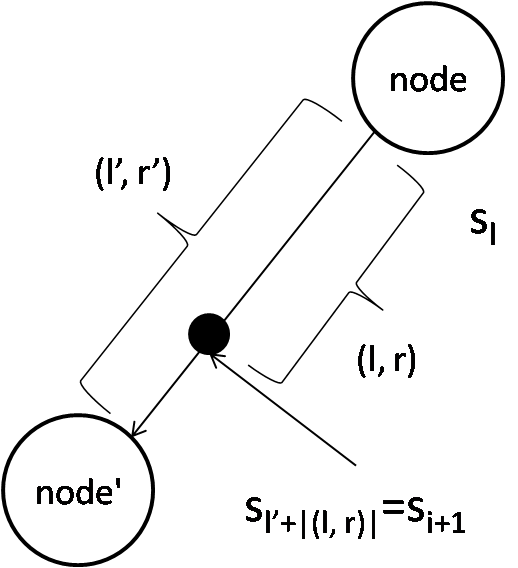
\includegraphics[scale=0.5]{img/implicit-end-point.eps}
     \caption{Implicit end point}
     \label{fig:implicit-end-point}
   \end{center}
\end{figure}

Ukkonen found a very important fact that if the $(node, (l, i))$ is the end
point of $SuffixTree(S_i)$, then $(node, (l, i+1))$ is the active point 
$SuffixTree(S_{i+1})$.

This is because if $(node, (l, i))$ is the end point of $SuffixTree(S_i)$,
It must have a $s_{i+1}$-child (either explicitly or implicitly).
If the suffix this end point represents is $s_ks_{k+1}...s_i$, it is the longest
suffix in $SuffxiTree(S_i)$ which satisfies $s_ks_{k+1}...s_is_{i+1}$ is a substring
of $S_i$. Consider $S_{i+1}$, $s_ks_{k+1}...s_is_{i+1}$ must occurs at least
twice in $S_{i+1}$, so position $(node, (l, i+1))$ is the active point of
$SuffixTree(S_{i+1})$. Figure \ref{fig:ep-ap} shows about this truth.

\begin{figure}[htbp]
   \begin{center}
     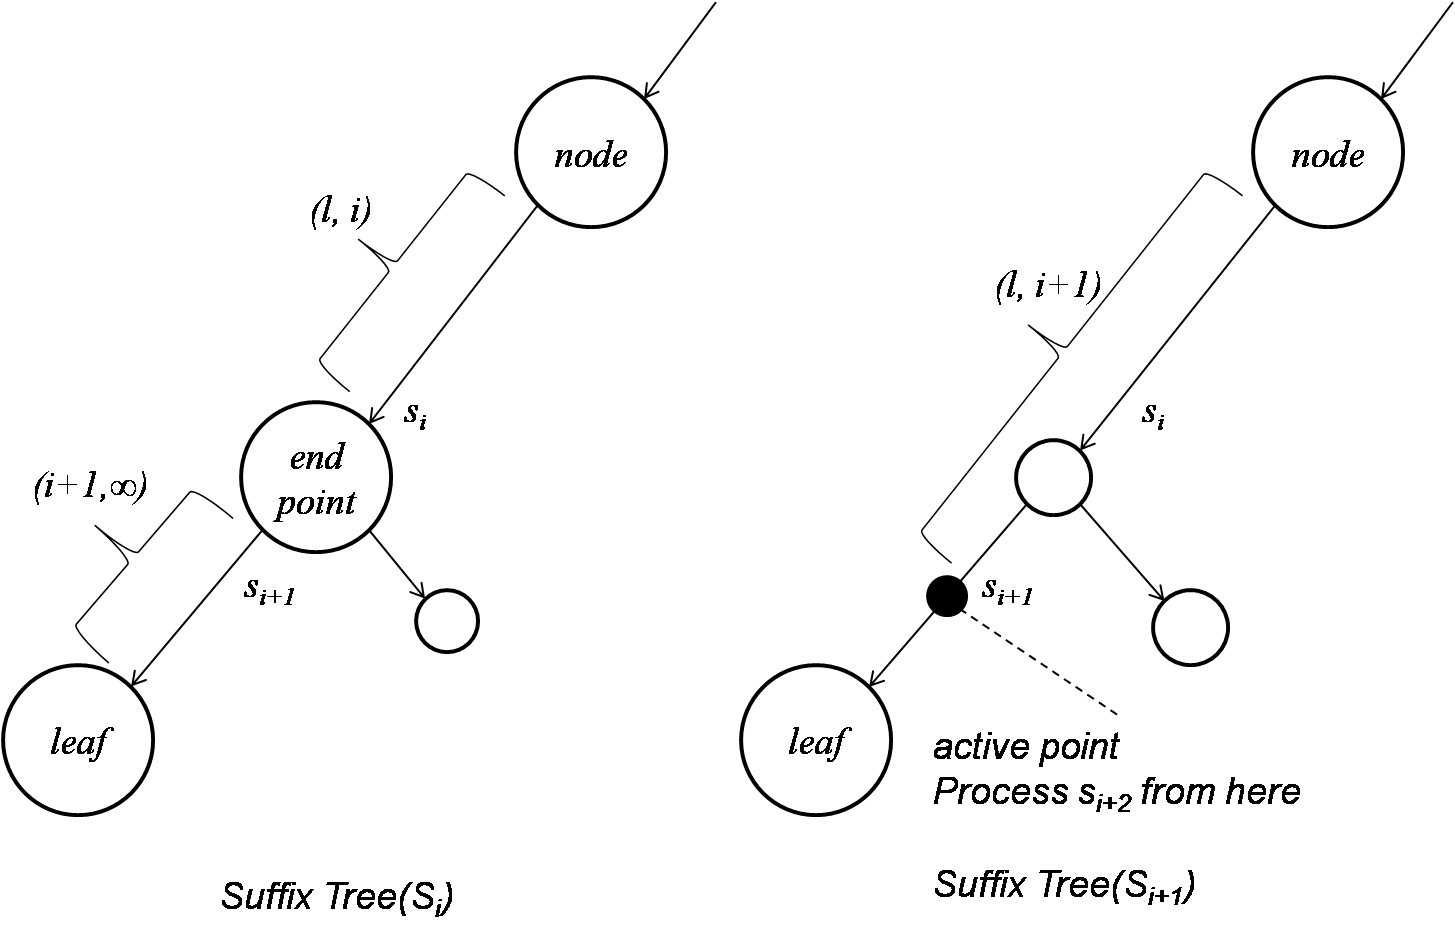
\includegraphics[scale=0.5]{img/ep-ap.eps}
     \caption{End point in $SuffixTree(S_i)$ and active point in $SuffixTree(S_{i+1})$.}
     \label{fig:ep-ap}
   \end{center}
\end{figure}

At this time point, the algorithm of Ukkonen's on-line construction can 
be given as the following.

%\begin{algorithm}
\begin{algorithmic}
\STATE $UPDATE(node, (l, i))$
  \STATE $prev \leftarrow CREATE-NEW-NODE()$
  \WHILE{$TRUE$}
    \STATE $(finish, node') \leftarrow END-POINT-BRANCH?(node, (l, i-1), s_i)$
    \IF{$finish = TRUE$}
      \STATE $BREAK$
    \ENDIF
    \STATE $CHILDREN(node')[s_i] \leftarrow ((i, \infty), CREATE-NEW-NODE())$
    \STATE $SUFFIX-LINK(prev) \leftarrow node'$
    \STATE $prev \leftarrow node'$
    \STATE $(node, l) = CANONIZE(SUFFIX-LINK(node), (l, i-1))$
  \ENDWHILE
  \STATE $SUFFIX-LINK(prev) \leftarrow node$
  \RETURN $(node, l)$
\end{algorithmic}
%\caption{Update $SuffixTree(S_{i-1})$}
%\label{algo:update}
%\end{algorithm}

This algorithm takes a parameter as reference pair $(node, (l, i))$, note that
position $(node, (l, i-1)$ is the active point for $SuffixTree(S_{i-1})$.
Next we enter a loop, this loop will go along with the suffix link until it
found the current position $(node, (l, i-1))$ is the end point. If it is not
end point, the function $END-POINT-BRNACH?()$ will return a position, from 
where the new leaf node will be branch out.

$END-POINT-BRANCH?()$ algorithm is implemented as below.

%\begin{algorithm}
\begin{algorithmic}
\STATE $END-POINT-BRANCH?(node, (l, r), c)$
  \IF{$(l, r) = \epsilon$}
    \IF{$node = NIL$}
      \RETURN $(TRUE, root)$
    \ELSE
      \RETURN $(CHILDREN(node)[c] = NIL?, node)$
    \ENDIF
  \ELSE
    \STATE $((l', r'), node') \leftarrow CHILDREN(node)[s_l]$
    \STATE $pos \leftarrow l'+|(l, r)|$
    \IF{$s_{pos}=c$}
      \RETURN $(TRUE, node)$
    \ELSE
      \STATE $p \leftarrow CREATE-NEW-NODE()$
      \STATE $CHILDREN(node)[s_{l'}] \leftarrow ((l', pos-1), p)$
      \STATE $CHILDREN(p)[s_{pos}] \leftarrow ((pos, r'), node')$
      \RETURN $(FALSE, p)$
    \ENDIF
  \ENDIF
\end{algorithmic}
%\caption{Test if a position is end point and create explicit node for further branching.}
%\label{algo:branch}
%\end{algorithm}

If the position is $(root, \epsilon)$, which means we have gone along suffix links to
the root, we return $TRUE$ to indicate the updating can be finished for this round.
If the position is in form of $(node, \epsilon)$, it means the reference pair represents
an explicit node, we just test if this node has already $c$-child, where $c=s_i$. and
if not, we can just branching out a leaf from this node.

In other case, which means the position $(node, (l, r))$ points to a implicit node.
We need find the exact position next to it to see if it is $c$-child implicitly.
If yes, we meet a end point, the updating loop can be finished, else, we make
the position an explicit node, and return it for further branching.

With the previous defined $CANONIZE()$ funciton, we can finalize the Ukkonen's algorithm.

%\begin{algorithm}
\begin{algorithmic}
\STATE $SUFFIX-TREE(S)$
  \STATE $root \leftarrow CREATE-NEW-NODE()$
  \STATE $node \leftarrow root, l \leftarrow 0$
  \FOR{$i \leftarrow 1$ to $LENGTH(S)$}
    \STATE $(node, l) = UPDATE(node, (l, i))$
    \STATE $(node, l) = CANONIZE(node, (l, i))$
  \ENDFOR
  \RETURN $root$
\end{algorithmic}
%\caption{Main algorithm of Ukkonen's on-line construction for suffix tree.}
%\label{algo:ukkonen2}
%\end{algorithm}

Figure \ref{fig:cons-stree-cacao} shows the phases when constructing the
suffix tree for string ``cacao'' with Ukkonen's algorithm.

\begin{figure}[htbp]
   \begin{center}
     \includegraphics[scale=0.5]{img/strie-empty.ps}empty
     \includegraphics[scale=0.5]{img/stree-c.ps}``c''
     \includegraphics[scale=0.5]{img/stree-ca.ps}``ca''
     \includegraphics[scale=0.5]{img/stree-cac.ps}``cac'' \newline
     \includegraphics[scale=0.5]{img/stree-caca.ps}``caca''
     \includegraphics[scale=0.5]{img/stree-cacao.ps}``cacao''
     \caption{Construction of suffix tree for ``cacao'', the 6 phases are shown, only the last layer of suffix links are shown in dotted arrow.}
     \label{fig:cons-stree-cacao}
   \end{center}
\end{figure}

Note that it needn't setup suffix link for leaf nodes, only branch nodes
have been set suffix links.

\subsubsection{Implementation of Ukkonen's algorithm in imperative languages}
The 2 main features of Ukkonen's algorithm are intense use of suffix link and
on-line update. So it will be very suitable to implement in imperative lanaguage.

\subsubsection*{Ukkonen's algorithm in Python}
The node definition is as same as the suffix Trie, however, the exact meaning
for children field are not same.

\lstset{language=Python}
\begin{lstlisting}
class Node:
    def __init__(self, suffix=None):
        self.children = {} # 'c':(word, Node), where word = (l, r)
        self.suffix = suffix
\end{lstlisting}

The children for suffix tree actually represent to the node transition
with reference pair. if the trasition is 
$CHILDREN(node)[s_l] \leftarrow ((l, r) node')$, 
The key type of the children is the character, which is corresponding 
to $s_l$, the data; the data type of the children is the referene pair.

Because there is only one copy of the complete string, all substrings
are represent in $(left, right)$ pairs, and the leaf are open pairs
as $(left, \infty)$, so we provide a tree definition in Python as below.

\begin{lstlisting}
class STree:
    def __init__(self, s):
        self.str = s
        self.infinity = len(s)+1000
        self.root = Node()
\end{lstlisting}

The infinity is defined as the length of the string plus a big number, we'll
benifit from python's list[a:b] expression that if the right index exceed to the
length of the list, the result is from left to the end of the list.

For convenience, I provide 2 helper funcitons for later use.

\begin{lstlisting}
def substr(str, str_ref):
    (l, r)=str_ref
    return str[l:r+1]

def length(str_ref):
    (l, r)=str_ref
    return r-l+1
\end{lstlisting}

The main entry for Ukkonen's algorithm is implemented as the following.

\begin{lstlisting}
def suffix_tree(str):
    t = STree(str)
    node = t.root # init active point is (root, Empty)
    l = 0
    for i in range(len(str)):
        (node, l) = update(t, node, (l, i))
        (node, l) = canonize(t, node, (l, i))
    return t
\end{lstlisting}

In the main entry, we initialize the tree and let the node points to the
root, at this time point, the active point is $(root, \epsilon)$, which
is (root, (0, -1)) in Python. we pass the active point to update() function 
in a loop from the left most index to the right most index of the string.
Inside the loop, update() funciton returns the end point, and we need 
convert it to canonical reference pair for the next time update.

the update() function is realized like the following.

\begin{lstlisting}
def update(t, node, str_ref):
    (l, i) = str_ref 
    c = t.str[i] # current char
    prev = Node() # dummy init 
    while True:
        (finish, p) = branch(t, node, (l, i-1), c)
        if finish:
            break
        p.children[c]=((i, t.infinity), Node())
        prev.suffix = p
        prev = p
        # go up along suffix link
        (node, l) = canonize(t, node.suffix, (l, i-1))
    prev.suffix = node
    return (node, l)
\end{lstlisting}

Different with Ukkonen's original program, I didn't use sentinel node.
The reference passed in is $(node, (l, i)$, the active point is
$(node, (l, i-1))$ actually, we passed the active point to branch() 
function. If it is end point, branch() function will return true
as the first element in the result. we then terminate the loop immediately.
Otherwise, branch() function will return the node which need to branch
out a new leaf as the second element in the result. The program
then create the new leaf, set it as open pair, and then go up along
with suffix link. The prev variable first point to a dummy node,
this can simplify the logic, and it used to record the position along
the boundary path. by the end of the loop, we'll finish the last
updating of the suffix link and return the end point. Since the end
point is always in form of (node, (l, i-1)), only (node, l) is returned.

Function branch() is used to test if a position is the end point
and turn the implicit node to explict node if neccessary.

\begin{lstlisting}
def branch(t, node, str_ref, c):
    (l, r) = str_ref
    if length(str_ref)<=0: # (node, empty)
        if node is None: #_|_
            return (True, t.root)
        else:
            return ((c in node.children), node)
    else:
        ((l1, r1), node1) = node.children[t.str[l]]
        pos = l1+length(str_ref)
        if t.str[pos]==c:
            return (True, node)
        else:             # node--->branch_node--->node1
            branch_node = Node()
            node.children[t.str[l1]]=((l1, pos-1), branch_node)
            branch_node.children[t.str[pos]] = ((pos, r1), node1)
            return (False, branch_node)
\end{lstlisting}

Because I don't use sentinel node, the special case is handled
in the first if-clause.

The canonize() function helps to conver a reference pair to 
canonical reference pair.

\begin{lstlisting}
def canonize(t, node, str_ref):
    (l, r) = str_ref 
    if node is None:
        if length(str_ref)<=0:
            return (None, l)
        else:
            return canonize(t, t.root, (l+1, r))
    while l<=r: # str_ref is not empty
        ((l1, r1), child) = node.children[t.str[l]] # node--(l', r')-->child
        if r-l >= r1-l1: #node--(l',r')-->child--->...
            l += r1-l1+1 # remove |(l',r')| chars from (l, r)
            node = child 
        else:
            break
    return (node, l)
\end{lstlisting}

Before testing the suffix tree construction algorithm, some helper
functions to convert the suffix tree to human readable string are
given.

\begin{lstlisting}
def to_lines(t, node):
    if len(node.children)==0:
        return [""]
    res = []
    for c, (str_ref, tr) in sorted(node.children.items()):
        lines = to_lines(t, tr)
        edge_str = substr(t.str, str_ref)
        lines[0] = "|--"+edge_str+"-->"+lines[0]
        if len(node.children)>1:
            lines[1:] = map(lambda l: "|"+" "*(len(edge_str)+5)+l, lines[1:])
        else:
            lines[1:] = map(lambda l: " "+" "*(len(edge_str)+6)+l, lines[1:])
        if res !=[]:
            res.append("|")
        res += lines
    return res

def to_str(t):
    return "\n".join(to_lines(t, t.root))
\end{lstlisting}

They are quite similar to the helper functions for suffix Trie print. The different
part is mainly cause by the reference pair of string.

In order to verify the implementation, some very simple test cases are feed to the
algorithm as below.

\begin{lstlisting}
class SuffixTreeTest:
    def __init__(self):
        print "start suffix tree test"

    def run(self):
        strs = ["cacao", "mississippi", "banana$"] #$ speical terminator
        for s in strs:
            self.test_build(s)

    def test_build(self, str):
        for i in range(len(str)):
            self.__test_build(str[:i+1])


    def __test_build(self, str):
        print "Suffix Tree ("+str+"):\n", to_str(suffix_tree(str)),"\n"
\end{lstlisting}

Here is a result snippet which shows the construciton phases for string ``cacao''

\begin{verbatim}
Suffix Tree (c):
|--c--> 

Suffix Tree (ca):
|--a-->
|
|--ca--> 

Suffix Tree (cac):
|--ac-->
|
|--cac--> 

Suffix Tree (caca):
|--aca-->
|
|--caca--> 

Suffix Tree (cacao):
|--a-->|--cao-->
|      |
|      |--o-->
|
|--ca-->|--cao-->
|       |
|       |--o-->
|
|--o--> 
\end{verbatim}

The result is identical to the one which is shown in figure \ref{fig:cons-stree-cacao}.

\subsubsection*{Ukkonen's algorithm in C++}
\label{ukkonen-c++}
Ukkonen's algorithm has much use of pairs, including reference pair and 
substring index pair. Altough STL provided std::pair tool, it is lack of
variable binding ability, for example (x, y)=apair like assignment isn't
leggal C++ code. boost::tuple provides a hany tool, tie(). I'l given a mimic
tool like boost::tie so that we can bind two variables to a pair.

\lstset{language=C++}
\begin{lstlisting}
template<typename T1, typename T2>
struct Bind{
  Bind(T1& r1, T2& r2):x1(r1), x2(r2){}
  Bind(const Bind& r):x1(r.x1), x2(r.x2){}

  // Support implicit type conversion
  template<typename U1, typename U2>
  Bind& operator=(const std::pair<U1, U2>& p){
    x1 = p.first;
    x2 = p.second;
    return *this;
  }
  T1& x1;
  T2& x2;
};

template<typename T1, typename T2>
Bind<T1, T2> tie(T1& r1, T2& r2){ 
  return Bind<T1, T2>(r1, r2); 
}
\end{lstlisting}

With this tool, we can tie variables like the following.

\begin{lstlisting}
int l, r;
tie(l, r) = str_pair;
\end{lstlisting}

We define substring index pair and reference pair like below.
First is string index reference pair.

\begin{lstlisting}
struct StrRef: public std::pair<int, int>{
  typedef std::pair<int, int> Pair;
  static std::string str;
  StrRef():Pair(){}
  StrRef(int l, int r):Pair(l, r){}
  StrRef(const Pair& ref):Pair(ref){}

  std::string substr(){
    int l, r;
    tie(l, r) = *this;
    return str.substr(l, r);
  }

  int len(){ 
    int l, r;
    tie(l, r) = *this;
    return r-l+1; 
  }
};

std::string StrRef::str="";
\end{lstlisting}

Because there is only one copy of the complete string, a static variable
is used to store it. substr() function is used to convert a pair of left,
right index into the sub-string. Function len() is used to calculate the
length of a sub-string.

Ukkonen's reference pair is defined in the sameway.

\begin{lstlisting}
struct Node;

struct RefPair: public std::pair<Node*, StrRef>{
  typedef std::pair<Node*, StrRef> Pair;
  RefPair():Pair(){}
  RefPair(Node* n, StrRef s):Pair(n, s){}
  RefPair(const Pair& p):Pair(p){}
  Node* node(){ return first; }
  StrRef str(){ return second; }
};
\end{lstlisting}

With these definition, the node type of suffix tree
can be defined.

\begin{lstlisting}
struct Node{
  typedef std::string::value_type Key;
  typedef std::map<Key, RefPair> Children;

  Node():suffix(0){}
  ~Node(){
    for(Children::iterator it=children.begin();
        it!=children.end(); ++it)
      delete it->second.node();
  }

  Children children;
  Node* suffix;
};
\end{lstlisting}

The children of a node is defined as a map with reference pairs stored.
In order for easy memory management, a recursive approach is used.

The final suffix tree is defined with a string and a root node.

\begin{lstlisting}
struct STree{
  STree(std::string s):str(s), 
                       infinity(s.length()+1000), 
                       root(new Node){}

  ~STree() { delete root; }
  std::string str;
  int infinity;
  Node* root;
};
\end{lstlisting}

the infinity is defined as the length of the string plus a big number.
Infinity will be used for leaf node as the `open to append' meaning.

Next is the main entry of Ukkonen's algorithm.

\begin{lstlisting}
STree* suffix_tree(std::string s){
  STree* t=new STree(s);
  Node* node = t->root; // init active point as (root, empty)
  for(unsigned int i=0, l=0; i<s.length(); ++i){
    tie(node, l) = update(t, node, StrRef(l, i));
    tie(node, l) = canonize(t, node, StrRef(l, i));
  }
  return t;
}
\end{lstlisting}

The program start from the initialized active point, and repeatly
call update(), the returned end point will be canonized and used
for the next active point.

Function update() is implemented as below.

\begin{lstlisting}
std::pair<Node*, int> update(STree* t, Node* node, StrRef str){
  int l, i;
  tie(l, i)=str;
  Node::Key c(t->str[i]); //current char
  Node dummy, *p;
  Node* prev(&dummy);
  while((p=branch(t, node, StrRef(l, i-1), c))!=0){
    p->children[c]=RefPair(new Node(), StrRef(i, t->infinity));
    prev->suffix = p;
    prev = p;
    // go up along suffix link
    tie(node, l) = canonize(t, node->suffix, StrRef(l, i-1));
  }
  prev->suffix = node;
  return std::make_pair(node, l);
}
\end{lstlisting}

In this function, pair (node, (l, i-1)) is the real active point
position. It is fed to branch() funciton. If the position is
end point, branch will return NULL pointer, so the while loop
terminates. else a node for branching out a new leaf is returned.
Then the program will go up along with suffix links and update
the previous suffix link accordingly. The end point will be
returned as the result of this function.

Function branch() is implemented as the following.

\begin{lstlisting}
Node* branch(STree* t, Node* node, StrRef str, Node::Key c){
  int l, r;
  tie(l, r) = str;
  if(str.len()<=0){ // (node, empty)
    if(node && node->children.find(c)==node->children.end())
      return node;
    else
      return 0; // either node is empty (_|_), or is EP
  }
  else{
    RefPair rp = node->children[t->str[l]];
    int l1, r1;
    tie(l1, r1) = rp.str();
    int pos = l1+str.len();
    if(t->str[pos]==c)
      return 0;
    else{ // node--->branch_node--->node1
      Node* branch_node = new Node();
      node->children[t->str[l1]]=RefPair(branch_node, StrRef(l1, pos-1));
      branch_node->children[t->str[pos]] = RefPair(rp.node(), StrRef(pos, r1));
      return branch_node;
    }
  }
}
\end{lstlisting}

If the position is (NULL, empty), it means the program arrive at the
root position, NULL pointer is returned to indicate the updating can
be terminated. If the position is in form of $(node, \epsilon)$, it 
then check if the node has already a $s_i$-child. In other case, it
means the position point to a implicit node, we need extra process
to test if it is end point. If not, a spliting happens to convert the
implicit node to exmplicit one.

The function to cononize a reference pair is given below.

\begin{lstlisting}
std::pair<Node*, int> canonize(STree* t, Node* node, StrRef str){
  int l, r;
  tie(l, r)=str;
  if(!node)
    if(str.len()<=0)
      return std::make_pair(node, l);
    else
      return canonize(t, t->root, StrRef(l+1, r));
  while(l<=r){ //str isn't empty
    RefPair rp = node->children[t->str[l]];
    int l1, r1;
    tie(l1, r1) = rp.str();
    if(r-l >= r1-l1){
      l += rp.str().len(); // remove len() from (l, r)
      node = rp.node();
    }
    else
      break;
  }
  return std::make_pair(node, l);
}
\end{lstlisting}

In order to test the program, some helper functions are provided
to represent the suffix tree as string. Among them, some are very
common tools.

\begin{lstlisting}
// map (x+) coll in Haskell
// boost lambda: transform(first, last, first, x+_1)
template<class Iter, class T>
void map_add(Iter first, Iter last, T x){
  std::transform(first, last, first, 
                 std::bind1st(std::plus<T>(), x));
}

// x ++ y in Haskell
template<class Coll>
void concat(Coll& x, Coll& y){
  std::copy(y.begin(), y.end(), 
            std::insert_iterator<Coll>(x, x.end()));
}
\end{lstlisting}

map\_add() will add a value to every element in a collection.
concat can concatenate tow collections together.

the suffix tree to string function is finally provided like this.

\begin{lstlisting}
std::list<std::string> to_lines(Node* node){
  typedef std::list<std::string> Result;
  Result res;
  if(node->children.empty()){
    res.push_back("");
    return res;
  }
  for(Node::Children::iterator it = node->children.begin();
      it!=node->children.end(); ++it){
    RefPair rp = it->second;
    Result lns = to_lines(rp.node());
    std::string edge = rp.str().substr();
    *lns.begin() = "|--" + edge + "-->" + (*lns.begin());
    map_add(++lns.begin(), lns.end(), 
            std::string("|")+std::string(edge.length()+5, ' '));
    if(!res.empty())
      res.push_back("|");
    concat(res, lns);
  }
  return res;
}

std::string to_str(STree* t){
  StrRef::str = t->str;
  std::list<std::string> ls = to_lines(t->root);
  std::ostringstream s;
  std::copy(ls.begin(), ls.end(), 
            std::ostream_iterator<std::string>(s, "\n"));
  return s.str();
}
\end{lstlisting}

After that, the program can be verfified by some simple test cases.

\begin{lstlisting}
class SuffixTreeTest{
public:
  SuffixTreeTest(){
    std::cout<<"Start suffix tree test\n";
  }
  void run(){
    test_build("cacao");
    test_build("mississippi");
    test_build("banana$"); //$ as special terminator
  }
private:
  void test_build(std::string str){
    for(unsigned int i=0; i<str.length(); ++i)
      test_build_step(str.substr(0, i+1));
  }

  void test_build_step(std::string str){
    STree* t = suffix_tree(str);
    std::cout<<"Suffix Tree ("<<str<<"):\n"
             <<to_str(t)<<"\n";
    delete t;
  }
};
\end{lstlisting}

Below are sinippet of suffix tree construction phases.

\begin{verbatim}
Suffix Tree (b):
|--b-->

Suffix Tree (ba):
|--a-->
|
|--ba-->

Suffix Tree (ban):
|--an-->
|
|--ban-->
|
|--n-->

Suffix Tree (bana):
|--ana-->
|
|--bana-->
|
|--na-->

Suffix Tree (banan):
|--anan-->
|
|--banan-->
|
|--nan-->

Suffix Tree (banana):
|--anana-->
|
|--banana-->
|
|--nana-->

Suffix Tree (banana$):
|--$-->
|
|--a-->|--$-->
|      |
|      |--nan-->|--$-->
|      |        |
|      |        |--na$-->
|
|--banana$-->
|
|--nan-->|--$-->
|        |
|        |--na$-->
\end{verbatim}

\subsubsection{Functional algorithm for suffix tree construction}
Ukkonen's algorithm is in a manner of on-ling updating and suffix
link plays very important role. Such properties can't be realized
in a functinal approach. Giegerich and Kurtz found Ukkonen's algorithm
can be transformed to McCreight's algorithm\cite{GieKur97}. These
two and the algorithm found by Weiner are all $O(n)$-algorithms.
They also conjecture (although it isn't proved) that any sequential
suffix tree construction not base on the important concepts, such
as suffix links, active suffixes, etc., will fail to meet $O(n)$-criterion.

There is implemented in PLT/Scheme\cite{plt-stree} based on
Ukkonen's algorithm, However it updates suffix links during the 
processing, so it is not pure functinal approach.

A lazy suffix tree construction method is discussed in \cite{GieKur95}.
And this method is contribute to Haskell Hackage by Bryan O'Sullivan.
\cite{Hackage-STree}.

This method benifit from the lazy evaluation property of 
Haskell progrmming languages, so that the tree won't be constructed
untill it is traversed. However, I think it is still a kind of brute-force
method. In other functional programming languages such as ML.
It can't be $O(n)$ algorithm.

I will provide a pure brute-force implementation which is similar
but not 100\% same in this post.

\subsubsection*{Brute-force suffix tree construction in Haskell}

For brute-force implementation, we needn't suffix link at all. The definition
of suffix node is plain straightforward.

\lstset{language=Haskell}
\begin{lstlisting}
data Tr = Lf | Br [(String, Tr)] deriving (Eq, Show)
type EdgeFunc = [String]->(String, [String])
\end{lstlisting}

The edge function plays interesting role. it takes a list of strings,
and extract a prefix of these strings, the prefix may not be the
longest prefix, and empty string is also possible. Whether extract
the longest prefix or just return them trivially can be defiend by different
edge functions.

For easy implementation, we limit the character set as below.

\begin{lstlisting}
alpha = ['a'..'z']++['A'..'Z']
\end{lstlisting}

This is only for illustration purpose, only the English lower case and upper
case letters are included. We can of course includes other characters if neccessary.

The core algorithm is given in list comprehension style.

\begin{lstlisting}
lazyTree::EdgeFunc -> [String] -> Tr
lazyTree edge = build where
    build [[]] = Lf
    build ss = Br [(a:prefix, build ss') | 
                         a<-alpha, 
                         xs@(x:_) <-[[cs | c:cs<-ss, c==a]],
                         (prefix, ss')<-[edge xs]]
\end{lstlisting}

lazyTree function takes a list of string, it will generate a radix
tree (for example a Trie or a patricia) from these string.

It will categorize all strings with the first letter in several groups, 
and remove the first letter for each elements in every group.
For example, for the string list [``acac'', ``cac'', ``ac'', ``c'']
the categorized group will be [('a', [``cac'', ``c'']), ('c', [``ac'', ``''])].
For easy understanding, I left the first letter, and write the groups
as tuple. then all strings with same first letter (removed) will
be fed to edge function.

Different edge function produce different radix trees. The most trivial
one will build a Trie.

\begin{lstlisting}
edgeTrie::EdgeFunc
edgeTrie ss = ("", ss)
\end{lstlisting}

If the edge function extract the longest common prefix, then it will 
build a Paticia.

\begin{lstlisting}
-- ex: 
--   edgeTree ["an", "another", "and"] = ("an", ["", "other", "d"])
--   edgeTree ["bool", "foo", "bar"] = ("", ["bool", "foo", "bar"])
--
-- some helper comments
--   let awss@((a:w):ss) = ["an", "another", "and"]
--       (a:w) = "an",  ss = ["another", "and"]
--       a='a', w="n"
--       rests awss = w:[u| _:u<-ss] = ["n", "nother", "nd"]
--
edgeTree::EdgeFunc
edgeTree [s] = (s, [[]])
edgeTree awss@((a:w):ss) | null [c|c:_<-ss, a/=c] = (a:prefix, ss')
                         | otherwise              = ("", awss)
                         where (prefix, ss') = edgeTree (w:[u| _:u<-ss])
edgeTree ss = ("", ss) -- (a:w):ss can't be match <==> head ss == ""
\end{lstlisting}

We can build suffix Trie and suffix tree with the above two functions.

\begin{lstlisting}
suffixTrie::String->Tr
suffixTrie = lazyTree edgeTrie . tails -- or init . tails

suffixTree::String->Tr
suffixTree = lazyTree edgeTree . tails
\end{lstlisting}

Below snippet is the result of constructing suffix Trie/tree for
string ``mississippi''.

\begin{verbatim}
SuffixTree("mississippi")=Br [("i",Br [("ppi",Lf),("ssi",Br [("ppi",Lf),
("ssippi",Lf)])]),("mississippi",Lf),("p",Br [("i",Lf),("pi",Lf)]),("s",
Br [("i",Br [("ppi",Lf),("ssippi",Lf)]),("si",Br [("ppi",Lf),("ssippi",
Lf)])])]
SuffixTrie("mississippi")=Br [("i",Br [("p",Br [("p",Br [("i",Lf)])]),
("s",Br [("s",Br [("i",Br [("p",Br [("p",Br [("i",Lf)])]),("s",Br [("s",
Br [("i",Br [("p",Br [("p",Br [("i",Lf)])])])])])])])])]),("m",Br [("i",
Br [("s",Br [("s",Br [("i",Br [("s",Br [("s",Br [("i",Br [("p",Br [("p",
Br [("i",Lf)])])])])])])])])])]),("p",Br [("i",Lf),("p",Br [("i",Lf)])]),
("s",Br [("i",Br [("p",Br [("p",Br [("i",Lf)])]),("s",Br [("s",Br [("i",
Br [("p",Br [("p",Br [("i",Lf)])])])])])]),("s",Br [("i",Br [("p",Br 
[("p",Br [("i",Lf)])]),("s",Br [("s",Br [("i",Br [("p",Br [("p",Br 
[("i",Lf)])])])])])])])])]
\end{verbatim}

Function lazyTree is common for all radix trees, the normal Patricia
and Trie can also be constructed with it.

\begin{lstlisting}
trie::[String]->Tr
trie = lazyTree edgeTrie

patricia::[String]->Tr
patricia = lazyTree edgeTree
\end{lstlisting}

Let's test it with some simple cases.

\begin{lstlisting}
trie ["zoo", "bool", "boy", "another", "an", "a"]
patricia ["zoo", "bool", "boy", "another", "an", "a"]
\end{lstlisting}

The results are as below.

\begin{verbatim}
Br [("a",Br [("n",Br [("o",Br [("t",Br [("h",Br [("e",
Br [("r",Lf)])])])])])]),("b",Br [("o",Br [("o",Br [("l",Lf)]),
("y",Lf)])]),("z",Br [("o",Br [("o",Lf)])])]

Br [("another",Lf),("bo",Br [("ol",Lf),("y",Lf)]),("zoo",Lf)]
\end{verbatim}

This is reason why I think the method is brute-force.

\subsubsection*{Brute-force suffix tree construction in Scheme/Lisp}.

The Functional implementation in Haskell utilizes list comprehension, which
is a handy syntax tool. In Scheme/Lisp, we use functions instead.

In MIT scheme, there are special functions to manipulate strings, which
is a bit different from list. Below are helper functions to simulate
car and cdr function for string.

\lstset{language=lisp}
\begin{lstlisting}
(define (string-car s)
  (if (string=? s "")
      ""
      (string-head s 1)))

(define (string-cdr s)
  (if (string=? s "")
      ""
      (string-tail s 1)))
\end{lstlisting}

The edge functions will extract common prefix from a list of strings.
For Trie, only the first common character will be extracted.

\begin{lstlisting}
;; (edge-trie '("an" "another" "and"))
;;  ==> ("a" "n" "nother" "nd")
(define (edge-trie ss)
  (cons (string-car (car ss)) (map string-cdr ss)))
\end{lstlisting}

While for suffix tree, we need extract the longest common prefix.

\begin{lstlisting}
;; (edge-tree '("an" "another" "and"))
;;   ==> ("an" "" "other" "d")
(define (edge-tree ss)
  (cond ((= 1 (length ss)) (cons (car ss) '()))
	((prefix? ss)
	 (let* ((res (edge-tree (map string-cdr ss)))
		(prefix (car res))
		(ss1 (cdr res)))
	   (cons (string-append (string-car (car ss)) prefix) ss1)))
	(else (cons "" ss))))

;; test if a list of strings has common prefix
;; (prefix '("an" "another" "and")) ==> true
;; (prefix '("" "other" "d")) ==> false
(define (prefix? ss)
  (if (null? ss)
      '()
      (let ((c (string-car (car ss))))
	(null? (filter (lambda (s) (not (string=? c (string-car s))))
		       (cdr ss))))))
\end{lstlisting}

For some old version of MIT scheme, there isn't definition for
partition function, so I defined one like below.

\begin{lstlisting}
;; overwite the partition if not supprt SRFI 1
;; (partition (> 5) '(1 6 2 7 3 9 0))
;;   ==>((6 7 9) 1 2 3 0)
(define (partition pred lst)
  (if (null? lst)
      (cons '() '())
      (let ((res (partition pred (cdr lst))))
	(if (pred (car lst))
	    (cons (cons (car lst) (car res)) (cdr res))
	    (cons (car res) (cons (car lst) (cdr res)))))))
\end{lstlisting}

Function groups can group a list of strings based on the first
letter of each string.

\begin{lstlisting}
;; group a list of strings based on first char
;; ss shouldn't contains "" string, so filter should be done first.
;; (groups '("an" "another" "bool" "and" "bar" "c"))
;;  ==> (("an" "another" "and") ("bool" "bar") ("c"))
(define (groups ss)
  (if (null? ss) 
      '()
      (let* ((c (string-car (car ss)))
	     (res (partition (lambda (x) (string=? c (string-car x))) (cdr ss))))
	(append (list (cons (car ss) (car res)))
		(groups (cdr res))))))
\end{lstlisting}

Function remove-empty can remove the empty string from the string list.

\begin{lstlisting}
(define (remove-empty ss)
  (filter (lambda (s) (not (string=? "" s))) ss))
\end{lstlisting}

With all the above tools, the core brute-force algorithm can be implemented
like the following.

\begin{lstlisting}
(define (make-tree edge ss)
  (define (bld-group grp)
    (let* ((res (edge grp))
	   (prefix (car res))
	   (ss1 (cdr res)))
      (cons prefix (make-tree edge ss1))))
  (let ((ss1 (remove-empty ss)))
    (if (null? ss1) '()
	(map bld-group (groups ss1)))))
\end{lstlisting}

The final suffix tree and suffix Trie construction algorithms can
be given.

\begin{lstlisting}
(define (suffix-tree s)
  (make-tree edge-tree (tails s)))

(define (suffix-trie s)
  (make-tree edge-trie (tails s)))
\end{lstlisting}

Below snippet are quick verification of this program.

\begin{lstlisting}
(suffix-trie "cacao") 
;Value 66: (("c" ("a" ("c" ("a" ("o"))) ("o"))) ("a" ("c" ("a" ("o"))) ("o")) ("o")) 
(suffix-tree "cacao") 
;Value 67: (("ca" ("cao") ("o")) ("a" ("cao") ("o")) ("o")) 
\end{lstlisting}

% ================================================================
%               Suffix tree applications
% ================================================================

\section{Suffix tree applications}

Suffix tree can help to solve a lot of string/DNA manipulation problems
paticularly fast. For typical problems will be list in this section.

\subsection{String/Pattern searching}
\label{substring-lookup}

There a plenty of string searching problems, among them includes the
famous KMP algorithm. Suffix tree can perform same level as 
KMP\cite{zhang-shaojie-lec}, that string searching in $O(m)$ complexity, 
where $m$ is the length of the substring.However, O(n) time is 
required to build the suffix tree in advance\cite{lallison-stree}.

Not only substring searching, but also pattern matching, including
regular expression matching can be solved with suffix tree. Ukkonen
summarize this kind of problems as substring motifs, and he gave the
result that {\em For a string $S$, $SuffixTree(S)$ gives complete occurrence 
counts of all substring motifs of $S$ in $O(n)$ time, although $S$ may have
$O(n^2)$ substrings.}

Note the facts of a $SuffixTree(S)$ that all internal nodes is corresponding
to a repeating substring of $S$ and the number of leaves of the sub-tree of a
node for string $P$ is the number of occurrence of $P$ in $S$.\cite{ukkonen-lec}

\subsubsection{Find the number of substring occurrence in imperative approach}

\subsubsection*{Find number of substring occurrence in Python}

The searching algorithm is almost as same as the Patricia looking 
up \cite{lxy-trie}. In Ukkonen's algorithm, there is only one copy
of string, and all edges are represent with index pairs. There are
some changes because of this reason. 

\lstset{language=Python}
\begin{lstlisting}
def lookup_pattern(t, node, s):
    f = (lambda x: 1 if x==0 else x)
    for _, (str_ref, tr) in node.children.items():
        edge = t.substr(str_ref)
        if string.find(edge, s)==0: #s `isPrefixOf` edge
            return f(len(tr.children))
        elif string.find(s, edge)==0: #edge `isPrefixOf` s
            return lookup_pattern(t, tr, s[len(edge):])
    return 0 # not found
\end{lstlisting}

I added a member function in STree to convert a string index
pair to string as below.

\begin{lstlisting}
class STree:
    #...
    def substr(self, sref):
        return substr(self.str, sref)
\end{lstlisting}

In lookup\_pattern() function, it takes a suffix tree which 
is built from the string.
A node is passed as the position to be looked up, it is root node when 
starting. Parameter s is the string to be searched.

The algorithm iterate all children of the node, it convert the string
index reference pair to edge substring, and check if s is prefix of the
the edge string, if matches, then the program can be terminated, the
number of the branches of this node will be returned as the number
of the occurrence of this substring. Note that no branch means there 
is only 1 occurrence. In case the edge is prefix of s, we then
recursively call the function to continue searching.

Because construction of the suffix tree is expensive, so we only 
do it when neccessary. We can do a lazy initialization as below.

\begin{lstlisting}
TERM1 = '$' # $: special terminator

class STreeUtil:
    def __init__(self):
        self.tree = None

    def find_pattern(self, str, pattern):
        if self.tree is None or self.tree.str!=str+TERM1:
            self.tree = stree.suffix_tree(str+TERM1)
        return lookup_pattern(self.tree, self.tree.root, pattern)
\end{lstlisting}

We always append special terminator to the string, so that there won't
be any suffix becomes the prefix of the other\cite{wiki-suffix-tree}.

Some simple test cases are given to verify the program.

\begin{lstlisting}
class StrSTreeTest:
    def run(self):
        self.test_find_pattern()

    def test_find_pattern(self):
        util=STreeUtil()
        self.__test_pattern__(util, "banana", "ana")
        self.__test_pattern__(util, "banana", "an")
        self.__test_pattern__(util, "banana", "anan")
        self.__test_pattern__(util, "banana", "nana")
        self.__test_pattern__(util, "banana", "ananan")

    def __test_pattern__(self, u, s, p):
        print "find pattern", p, "in", s, ":", u.find_pattern(s, p)
\end{lstlisting}

And the output is like the following.

\begin{verbatim}
find pattern ana in banana : 2
find pattern an in banana : 2
find pattern anan in banana : 1
find pattern nana in banana : 1
find pattern ananan in banana : 0
\end{verbatim}

\subsubsection*{Find the number of substring occurrence in C++}
TODO:

\subsubsection{Find the number of substring occurrence in functional approach}
TODO:

\subsubsection*{Find the number of substring occurrence in Haskell}
TODO:

\subsubsection*{Find the number of substring occurrence in Scheme/Lisp}
TODO:

\subsubsection{Complete pattern search}
For search pattern like ``a**n'' with suffix tree, please refer to \cite{ukkonen-lec} and \cite{ukkonen-search}.

\subsection{Find the longest repeated substring}

If we go one step ahead from \ref{substring-lookup}, below result can
be found.

{\em After adding a special terminater character to string S, The 
longest repeated substring can be found by searching the 
deepest branches in suffix tree.}

Consider the example suffix tree shown in figure \ref{fig:stree-mississippis}

\begin{figure}[htbp]
   \begin{center}
      \includegraphics[scale=0.5]{img/stree-mississippis.ps}
      \caption{The suffix tree for `mississippi\$'} \label{fig:stree-mississippis}
   \end{center}
\end{figure}

There are 3 branch nodes, A, B, and C which depth is 3. However, A represents
the longest repeated substring ``issi''. B and C represent for ``si'', ``ssi'',
they are all shorter than A. 

This example tells us that the ``depth'' of the branch node should be measured
by the number of characters traversed from the root.

\subsubsection{Find the longest repeated substring in imperative approach}
According to the above analysis, to find the longest repeated substring
can be turned into a BFS (Bread First Search) in a suffix tree.

\begin{algorithmic}
\STATE $LONGEST-REPEATED-SUBSTRING(T)$
  \STATE $Q \leftarrow {NIL, ROOT(T)}$
  \STATE $R \leftarrow NIL$
  \WHILE{$Q$ is not empty}
    \STATE $(s, node) \leftarrow POP(Q)$
    \FOR{each $((l, r), node')$ in $CHILDREN(node)$}
      \IF{$node'$ is not leaf}
        \STATE $s' \leftarrow CONCATENATE(s, (l, r))$
        \STATE $PUSH(Q, {s', node'})$
        \STATE $UPDATE(R, s')$
      \ENDIF
    \ENDFOR
  \ENDWHILE
  \RETURN $R$
\end{algorithmic}

where algorithm $UPDATE()$ will compare the longest repeated substring
candidates. If two candidates have the same length, one simple solution
is just take one as the final result, the other solution is to maintain
a list contains all candidates with same length.

\begin{algorithmic}
\STATE $UPDATE(l, x)$
  \IF{$l = NIL$ or $LENGTH(l[1]) < LENGTH(x)$}
    \RETURN $l \leftarrow [x]$
  \ELSIF {$LENGTH(l[1]) = LENGTH(x)$}
    \RETURN $APPEND(l, x)$
  \ENDIF
\end{algorithmic}

Note that the index of a list starts from 1 in this algorithm.

\subsubsection*{Find the longest repeated substring in Python}
The above algorithm can be translated into Python program as the following.

\lstset{language=Python}
\begin{lstlisting}
def lrs(t):
    queue = [("", t.root)]
    res = []
    while len(queue)>0:
        (s, node) = queue.pop(0)
        for _, (str_ref, tr) in node.children.items():
            if len(tr.children)>0:
                s1 = s+t.substr(str_ref)
                queue.append((s1, tr))
                res = update_max(res, s1)
    return res

def update_max(lst, x):
    if lst ==[] or len(lst[0]) < len(x):
        return [x]
    elif len(lst[0]) == len(x):
        return lst + [x]
    else:
        return lst
\end{lstlisting}

In order to verify this program, some simple test cases are fed.

\begin{lstlisting}
class StrSTreeTest:
    #...

    def run(self):
        #...
        self.test_lrs()

    def test_lrs(self):
        self.__test_lrs__("mississippi")
        self.__test_lrs__("banana")
        self.__test_lrs__("cacao")
        self.__test_lrs__("foofooxbarbar")

    def __test_lrs__(self, s):
        print "longest repeated substrings of", s, "=", self.util.find_lrs(s)
\end{lstlisting}

By running the test case, the result like below can be obtained.

\begin{verbatim}
find pattern ananan in banana : 0
longest repeated substrings of mississippi = ['issi']
longest repeated substrings of banana = ['ana']
longest repeated substrings of cacao = ['ca']
longest repeated substrings of foofooxbarbar = ['bar', 'foo']
\end{verbatim}

\subsubsection{Find the longest repeated substring in functional approach}
TODO:

\subsubsection*{Find the longest repeated substring in Haskell}
TODO:

\subsection{Find the longest common substring}
TODO:

\subsection{Find the longest palindrome in a string}
TODO:

\subsection{Others}
TODO: Data compression, Burrows-Wheeler transform, LZW compression (LZSS)
etc.

% ================================================================
%                 Short summary
% ================================================================
\section{Notes and short summary}

Suffix Tree was first introduced by Weiner in 1973 \cite{weiner}.

TODO: Short summary here.

% ================================================================
%                 Appendix
% ================================================================
\section{Appendix} \label{appendix}
%\appendix
All programs provided along with this article are free for
downloading.

\subsection{Prerequisite software}
GNU Make is used for easy build some of the program. For C++ and ANSI C programs,
GNU GCC and G++ 3.4.4 are used. I use boost triple to reduce the
amount of our code lines, boost library version I am using is
1.33.1. The path is in CXX variable in Makefile, please change it to
your path when compiling.
For Haskell programs GHC 6.10.4 is used
for building. For Python programs, Python 2.5 is used for testing, for
Scheme/Lisp program, MIT Scheme 14.9 is used.

all source files are put in one folder. Invoke 'make' or 'make all'
will build C++ and Haskell program. 

Run 'make Haskell' will separate build Haskell program. There will be
two executable file generated one is htest the other is happ (with .exe
in Window like OS). Run htest will test functions in ...

\subsection{Tools}

Besides them, I use graphviz to draw most of the figures in this post. In order to
translate the Trie, Patrica and Suffix Tree output to dot language scripts. I wrote a python program.
it can be used like this.

\begin{verbatim}
st2dot...
\end{verbatim}

This helper scripts can also be downloaded with this article.

download position: http://sites.google.com/site/algoxy/stree/stree.zip

\begin{thebibliography}{99}

\bibitem{ukkonen95}
Esko Ukkonen. ``On-line construction of suffix trees''. Algorithmica 14 (3): 249--260. doi:10.1007/BF01206331. http://www.cs.helsinki.fi/u/ukkonen/SuffixT1withFigs.pdf

\bibitem{wiki-suffix-tree}
Suffix Tree, Wikipedia. http://en.wikipedia.org/wiki/Suffix\_tree

\bibitem{ukkonen-presentation}
Esko Ukkonen. ``Suffix tree and suffix array techniques for pattern ananlysis in strings''. http://www.cs.helsinki.fi/u/ukkonen/Erice2005.ppt

\bibitem{wiki-trie}
Trie, Wikipedia. http://en.wikipedia.org/wiki/Trie

\bibitem{lxy-trie}
Liu Xinyu. ``Trie and Patricia, with Functional and imperative implementation''. http://sites.google.com/site/algoxy/trie

\bibitem{trivial-stree-java}
Suffix Tree (Java). http://en.literateprograms.org/Suffix\_tree\_(Java)

\bibitem{GieKur97}
Robert Giegerich and Stefan Kurtz. ``From Ukkonen to McCreight and Weiner: A Unifying View of Linear-Time Suffix Tree Construction''. Science of Computer Programming 25(2-3):187-218, 1995. http://citeseer.ist.psu.edu/giegerich95comparison.html

\bibitem{GieKur95}
Robert Giegerich and Stefan Kurtz. ``A Comparison of Imperative and Purely Functional Suffix Tree Constructions''. Algorithmica 19 (3): 331--353. doi:10.1007/PL00009177. www.zbh.uni-hamburg.de/pubs/pdf/GieKur1997.pdf

\bibitem{Hackage-STree}
Bryan O'Sullivan. ``suffixtree: Efficient, lazy suffix tree implementation''. http://hackage.haskell.org/package/suffixtree

\bibitem{plt-stree}
Danny. http://hkn.eecs.berkeley.edu/~dyoo/plt/suffixtree/

\bibitem{zhang-shaojie-lec}
Zhang Shaojie. ``Lecture of Suffix Trees''. http://www.cs.ucf.edu/~shzhang/Combio09/lec3.pdf

\bibitem{lallison-stree}
Lloyd Allison. ``Suffix Trees''. http://www.allisons.org/ll/AlgDS/Tree/Suffix/

\bibitem{ukkonen-lec}
Esko Ukkonen. ``Suffix tree and suffix array techniques for pattern analysis in strings''. http://www.cs.helsinki.fi/u/ukkonen/Erice2005.ppt

\bibitem{ukkonen-search}
Esko Ukkonen ``Approximate string-matching over suffix trees''. Proc. CPM 93. Lecture Notes in Computer Science 684, pp. 228-242, Springer 1993. http://www.cs.helsinki.fi/u/ukkonen/cpm931.ps

\end{thebibliography}

\ifx\wholebook\relax \else
\end{document}
\fi
